\documentclass[a4paper,14pt]{extarticle}

\usepackage[utf8x]{inputenc}
\usepackage[T1]{fontenc}
\usepackage[russian]{babel}
\usepackage{hyperref}
\usepackage{indentfirst}
\usepackage{here}
\usepackage{array}
\usepackage{graphicx}
\usepackage{caption}
\usepackage{subcaption}
\usepackage{chngcntr}
\usepackage{amsmath}
\usepackage{amssymb}
\usepackage[left=2cm,right=2cm,top=2cm,bottom=2cm,bindingoffset=0cm]{geometry}
\usepackage{multicol}
\usepackage{multirow}
\usepackage{titlesec}
\usepackage{listings}
\usepackage{color}
\usepackage{enumitem}
\usepackage{cmap}
\usepackage{url}

\definecolor{green}{rgb}{0,0.6,0}
\definecolor{gray}{rgb}{0.5,0.5,0.5}
\definecolor{purple}{rgb}{0.58,0,0.82}

\lstdefinelanguage{none}{}

\lstset{
	language={none},
	inputpath={../logs/},
	backgroundcolor=\color{white},
	commentstyle=\color{green},
	keywordstyle=\color{blue},
	numberstyle=\color{gray}\scriptsize\ttfamily,
	stringstyle=\color{purple},
	basicstyle=\footnotesize\ttfamily,
	breakatwhitespace=false,
	breaklines=true,
	captionpos=b,
	keepspaces=true,
	numbers=left,
	numbersep=5pt,
	showspaces=false,
	showstringspaces=false,
	showtabs=false,
	tabsize=4,
	frame=single,
	morekeywords={},
	deletekeywords={},
	extendedchars=false,
	columns=fullflexible,
	literate=%
		{~}{{\raise.25ex\hbox{$\mathtt{\sim}$}}}{1}%
		{-}{-}{1}
}

\titleformat*{\section}{\large\bfseries} 
\titleformat*{\subsection}{\normalsize\bfseries} 
\titleformat*{\subsubsection}{\normalsize\bfseries} 
\titleformat*{\paragraph}{\normalsize\bfseries} 
\titleformat*{\subparagraph}{\normalsize\bfseries} 

\counterwithin{figure}{section}
\counterwithin{equation}{section}
\counterwithin{table}{section}
\newcommand{\sign}[1][5cm]{\makebox[#1]{\hrulefill}}
\newcommand{\equipollence}{\quad\Leftrightarrow\quad}
\newcommand{\no}[1]{\overline{#1}}
\graphicspath{{../pics/}}
\captionsetup{justification=centering,margin=1cm}
\def\arraystretch{1.3}
\setlength\parindent{5ex}
\titlelabel{\thetitle.\quad}

\setitemize{topsep=0em, itemsep=0em}
\setenumerate{topsep=0em, itemsep=0em}

\begin{document}

\begin{titlepage}
\begin{center}
	Санкт-Петербургский Политехнический Университет Петра Великого\\[0.3cm]
	Институт компьютерных наук и технологий \\[0.3cm]
	Кафедра компьютерных систем и программных технологий\\[4cm]
	
	\textbf{ОТЧЕТ}\\ 
	\textbf{по лабораторной работе}\\[0.5cm]
	\textbf{<<Data Mining>>}\\[0.1cm]
	Интеллектуальные системы\\[3.0cm]
\end{center}

\begin{flushright}
	\begin{minipage}{0.5\textwidth}
		\textbf{Работу выполнил студент}\\[3mm]
		гр. 3540901/91502 \hfill \sign[1.1cm] \hfill Дьячков В.В.\\[5mm]
		\textbf{Работу принял преподаватель}\\[5mm]
		\sign[2.1cm] \hfill к.т.н., доц. Бендерская Е.Н. \\[5mm]
	\end{minipage}
\end{flushright}

\vfill

\begin{center}
	Санкт-Петербург\\[0.3cm]
	\the\year
\end{center}
\end{titlepage}

\addtocounter{page}{1}

\tableofcontents
\newpage

\section{Программа работы}

\begin{enumerate}
	\item Ознакомьтесь с методическим пособием Татжибаева О.А. Разработка экспертных систем [Текст]: методические указания к расчетно-графическим работам по дисциплине
	«Системы искусственного интеллекта»\cite{tatj}.
	\item Разработайте экспертную систему в соответствии с вариантами заданий на стр. 23-30 в	пособии.
	\item Можно ли решить поставленную задачу проще без использования ЭС?
	\item В каких областях, по Вашему мнению, использование ЭС потенциально опасно (или вредно)?
\end{enumerate}

\section{Разработка ЭС}

\noindent Экспертная система по выбору оператора сотовой связи. Входные данные:

\begin{enumerate}
	\item зона уверенного приема сигнала;
	\item стоимость роуминга;
	\item предоставляемые услуги SMS, MMS, WAP
	\item тарифные планы.
\end{enumerate}

\subsection{Переменные}

Разработанная экспертная система включает в себя переменные типа \code{Static list}, отражающие критерии выбора оператора, переменную типа \code{Numeric} для стоимости роуминга, и переменные типа \code{Confidence}, использующиеся как возможные операторы сотовой связи (Теле2, МТС и Билайн).

\begin{table}[H]
	\centering
	\caption{Список переменных}
	\begin{tabular}{|c|l|c|}
		\hline
		Тип & \multicolumn{1}{c|}{Название} & Значение \\ \hline
		\multirow{3}{*}{\code{Static list}}
		& \code{Zone} (Зона обслуживания) & \code{[Country, World]}  \\ \cline{2-3}
		& \code{Service} (Включенные услуги) & \code{[SMS, MMS, MAP]}   \\ \cline{2-3}
		& \code{Tariff} (Тарифный план) & \code{[Gold, Silver]}    \\ \hline
		\code{Numeric} & \code{Price} (Стоимость роуминга) & Number \\ \hline
		\multirow{3}{*}{\code{Confidence}}
		& \code{Tele2}   & 10 \\ \cline{2-3}
		& \code{MTS}     & 10 \\ \cline{2-3}
		& \code{Beeline} & 10 \\ \hline
	\end{tabular}
\end{table}

\subsection{Дерево решений ЭС}

Приведем дерево решений разработанной ЭС.

\begin{figure}[H]
	\centering
	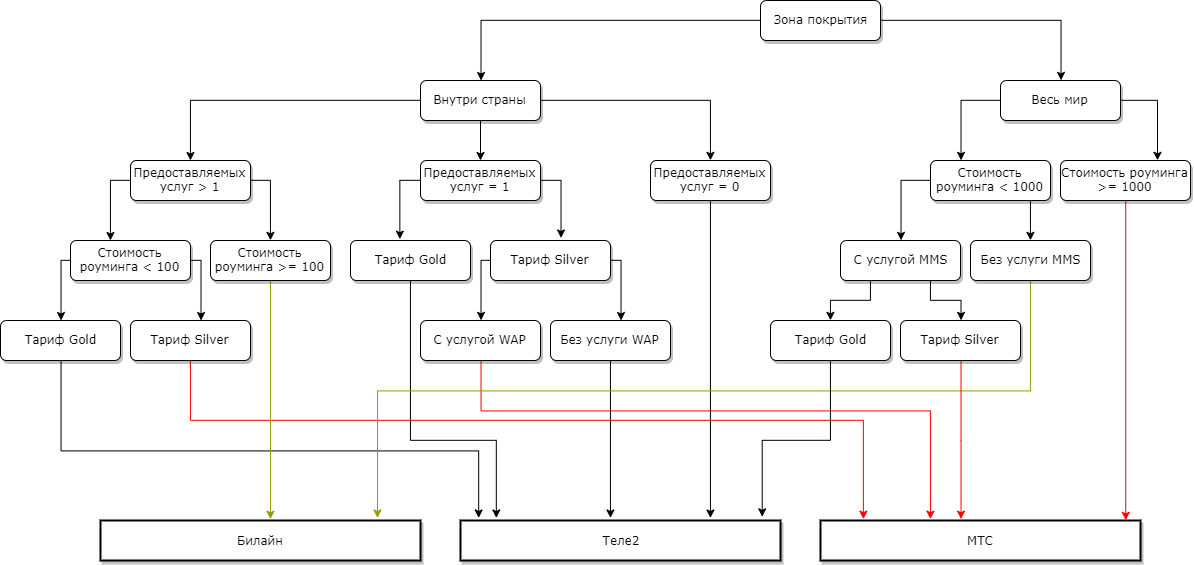
\includegraphics[height=0.6\linewidth,angle=-90]{tree}
	\caption{Дерево решений ЭС}
\end{figure}

\subsection{База знаний ЭС}

Приведем описание логического блока ЭС.

\begin{figure}[H]
	\centering
	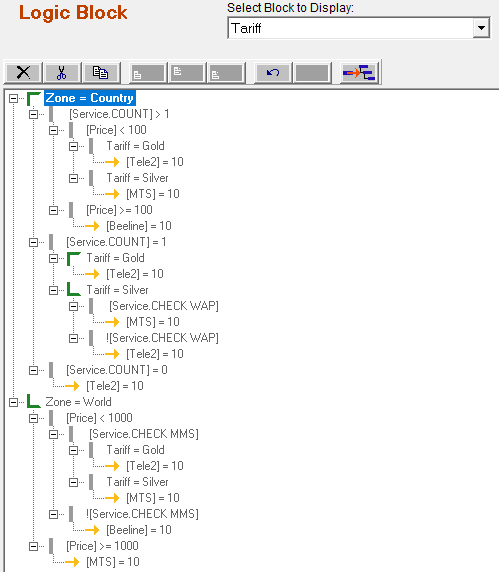
\includegraphics[width=0.7\linewidth]{logic}
	\caption{Логический блок ЭС}
\end{figure}

\begin{lstlisting}[caption={Алгоритм работы ЭС}]
IF:
	Zone Country
AND:
	[Service.COUNT] > 1
AND:
	[Price] < 100
AND:
	Tariff Gold
THEN:
	Tele2: Confidence = 10

IF:
	Zone Country
AND:
	[Service.COUNT] > 1
AND:
	[Price] < 100
AND:
	Tariff Silver
THEN:
	MTS: Confidence = 10


IF:
	Zone Country
AND:
	[Service.COUNT] > 1
AND:
	[Price] >= 100
THEN:
	Beeline: Confidence = 10

IF:
	Zone Country
AND:
	[Service.COUNT] = 1
AND:
	Tariff Gold
THEN:
	Tele2: Confidence = 10

IF:
	Zone Country
AND:
	[Service.COUNT] = 1
AND:
	Tariff Silver
AND: 
	[Service.CHECK WAP]
THEN:
	MTS: Confidence = 10

IF:
	Zone Country
AND:
	[Service.COUNT] = 1
AND:
	Tariff Silver
AND:
	![Service.CHECK WAP] 
THEN:
	Tele2: Confidence = 10

IF:
	Zone Country
AND:
	[Service.COUNT] = 0 
THEN:
	Tele2: Confidence = 10

IF:
	Zone World
AND:
	[Price] < 1000
AND:
	[Service.CHECK MMS]
AND:
	Tariff Gold
THEN:
	Tele2: Confidence = 10

IF:
	Zone World
AND:
	[Price] < 1000
AND:
	[Service.CHECK MMS]
AND:
	Tariff Silver
THEN:
	MTS: Confidence = 10

IF:
	Zone World
AND:
	[Price] < 1000
AND:
	![Service.CHECK MMS]
THEN:
	Beeline: Confidence = 10

IF:
	Zone World
AND:
	[Price] >= 1000
THEN:
	MTS: Confidence = 10
\end{lstlisting}

\subsection{Пользовательский интерфейс}

Для ЭС был разработан интерфейс, схожий с примерами из лабораторных работ.

\begin{figure}[H]
	\centering
	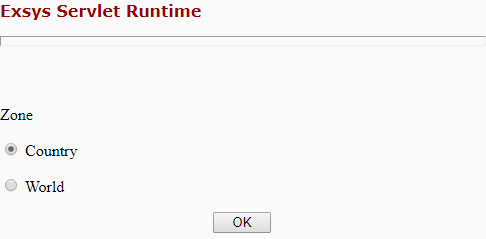
\includegraphics[width=0.7\linewidth]{tariff_1}
	\caption{Пример вопроса о зоне покрытия}
\end{figure}

\begin{figure}[H]
	\centering
	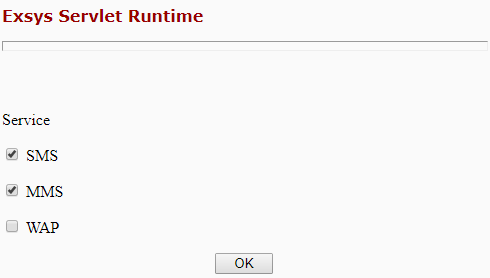
\includegraphics[width=0.7\linewidth]{tariff_2}
	\caption{Пример вопроса о включенных услугах}
\end{figure}


\begin{figure}[H]
	\centering
	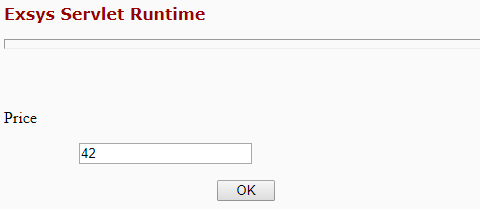
\includegraphics[width=0.7\linewidth]{tariff_3}
	\caption{Пример вопроса о стоимости роуминга}
\end{figure}

\begin{figure}[H]
	\centering
	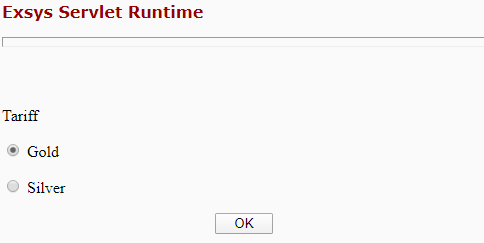
\includegraphics[width=0.7\linewidth]{tariff_4}
	\caption{Пример вопроса о тарифном плане}
\end{figure}

\begin{figure}[H]
	\centering
	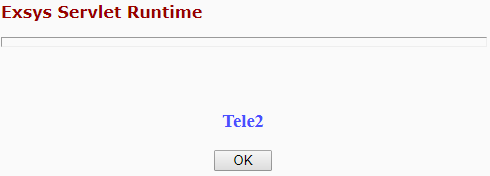
\includegraphics[width=0.7\linewidth]{tariff_5}
	\caption{Пример результата работы ЭС}
\end{figure}

\section{Выводы}

В ходе лабораторной работы была разработана экспертная система для выбора оператора сотовой связи. Полученная ЭС учитывает зону покрытия оператора, дополнительные услуги, тарифный план и стоимость роуминга. Из совокупности этих факторов составляется рекомендация, представляющая собой одного из операторов связи.

\paragraph{Можно ли решить поставленную задачу проще без использования ЭС?}

Задачу можно решить без помощи экспертной системы, однако временные затраты на создание такого решения могут увеличиться. В простом примере, как в рассмотренном выше, экспертная система играет роль инструмента для запроса из обычной базы данных с определенными параметрами (тариф, стоимость, услуги).  Тем не менее, для более сложного примера, ЭС может быть успешно использована благодаря механизму обратной связи с выведением фактом через наводящие вопросы пользователю.

\paragraph{В каких областях, по Вашему мнению, использование ЭС потенциально опасно (или вредно)?}

Опасность может представлять использование ЭС в областях, где от ее решения может зависеть жизнь человека (например, в медицине). Вредным (или излишним) может быть использование ЭС в областях, где накопленные знания быстро устаревают и теряю ценность.

\bibliographystyle{plain}
\addcontentsline{toc}{section}{Список литературы}
\bibliography{refs}

\end{document}
